% !TEX root = template.tex

\section{Results}
\label{sec:results}

Following the main approach in the KWS literature, we evaluate model performance based on the top-1 accuracy score on the test set. In Table \ref{table:results} we report all the results for each model and for each task. Additionally, in Figure \ref{fig:accs_vs_parameters} we provide a plot of each model accuracy against its number of parameters. The SQAtt-RNN provides a comparable accuracy for the 12kws task, while giving slightly worse results for the 35kws task. This suggests that providing a single query vector representative for the whole sequence is more than sufficient when dealing with relatively short sequences. Indeed, the query vector comes from a bidirectional GRU layer, which proved to be really good at capturing the relations between the sequence elements. The models based on multi head attention didn't provide consistent results: specifically, contrary to expectations, increasing the number of heads didn't necessarily increase the performances of the model. Nevertheless, the best scoring models were SQMHAtt-RNN5 for the 12kws task, and SQMHAtt-RNN2 for the 35kws task. While it is true that multi head attention models are heavier in terms of memory footprint with respect to Att-RNN, the ones proposed here still present less parameters than the one proposed in \cite{streamingkws2020Rybakov}, which reported to have around $700$K parameters.

In the same way, also the ResAtt models didn't provide consistent results, and in general seemed to perform worse than the simipler CNN block from Att-RNN. Maybe results in this sense can be improved employing more sophisticated recurrent blocks. Also, by looking at the performances of the SQ-noCNN model, it is interesting to note that for the 12kws task performance is slightly better with respect to Att-RNN, while for the 35kws task they are worse. This could suggest that the feature extraction task performed by the CNN block might be more important when in need to recognize an higher amount of key-words. In Figure We also provide a confusion matrix for the best performing models, for both tasks

\begin{figure*}
	\centering
	\begin{subfigure}{\textwidth}
		\centering
		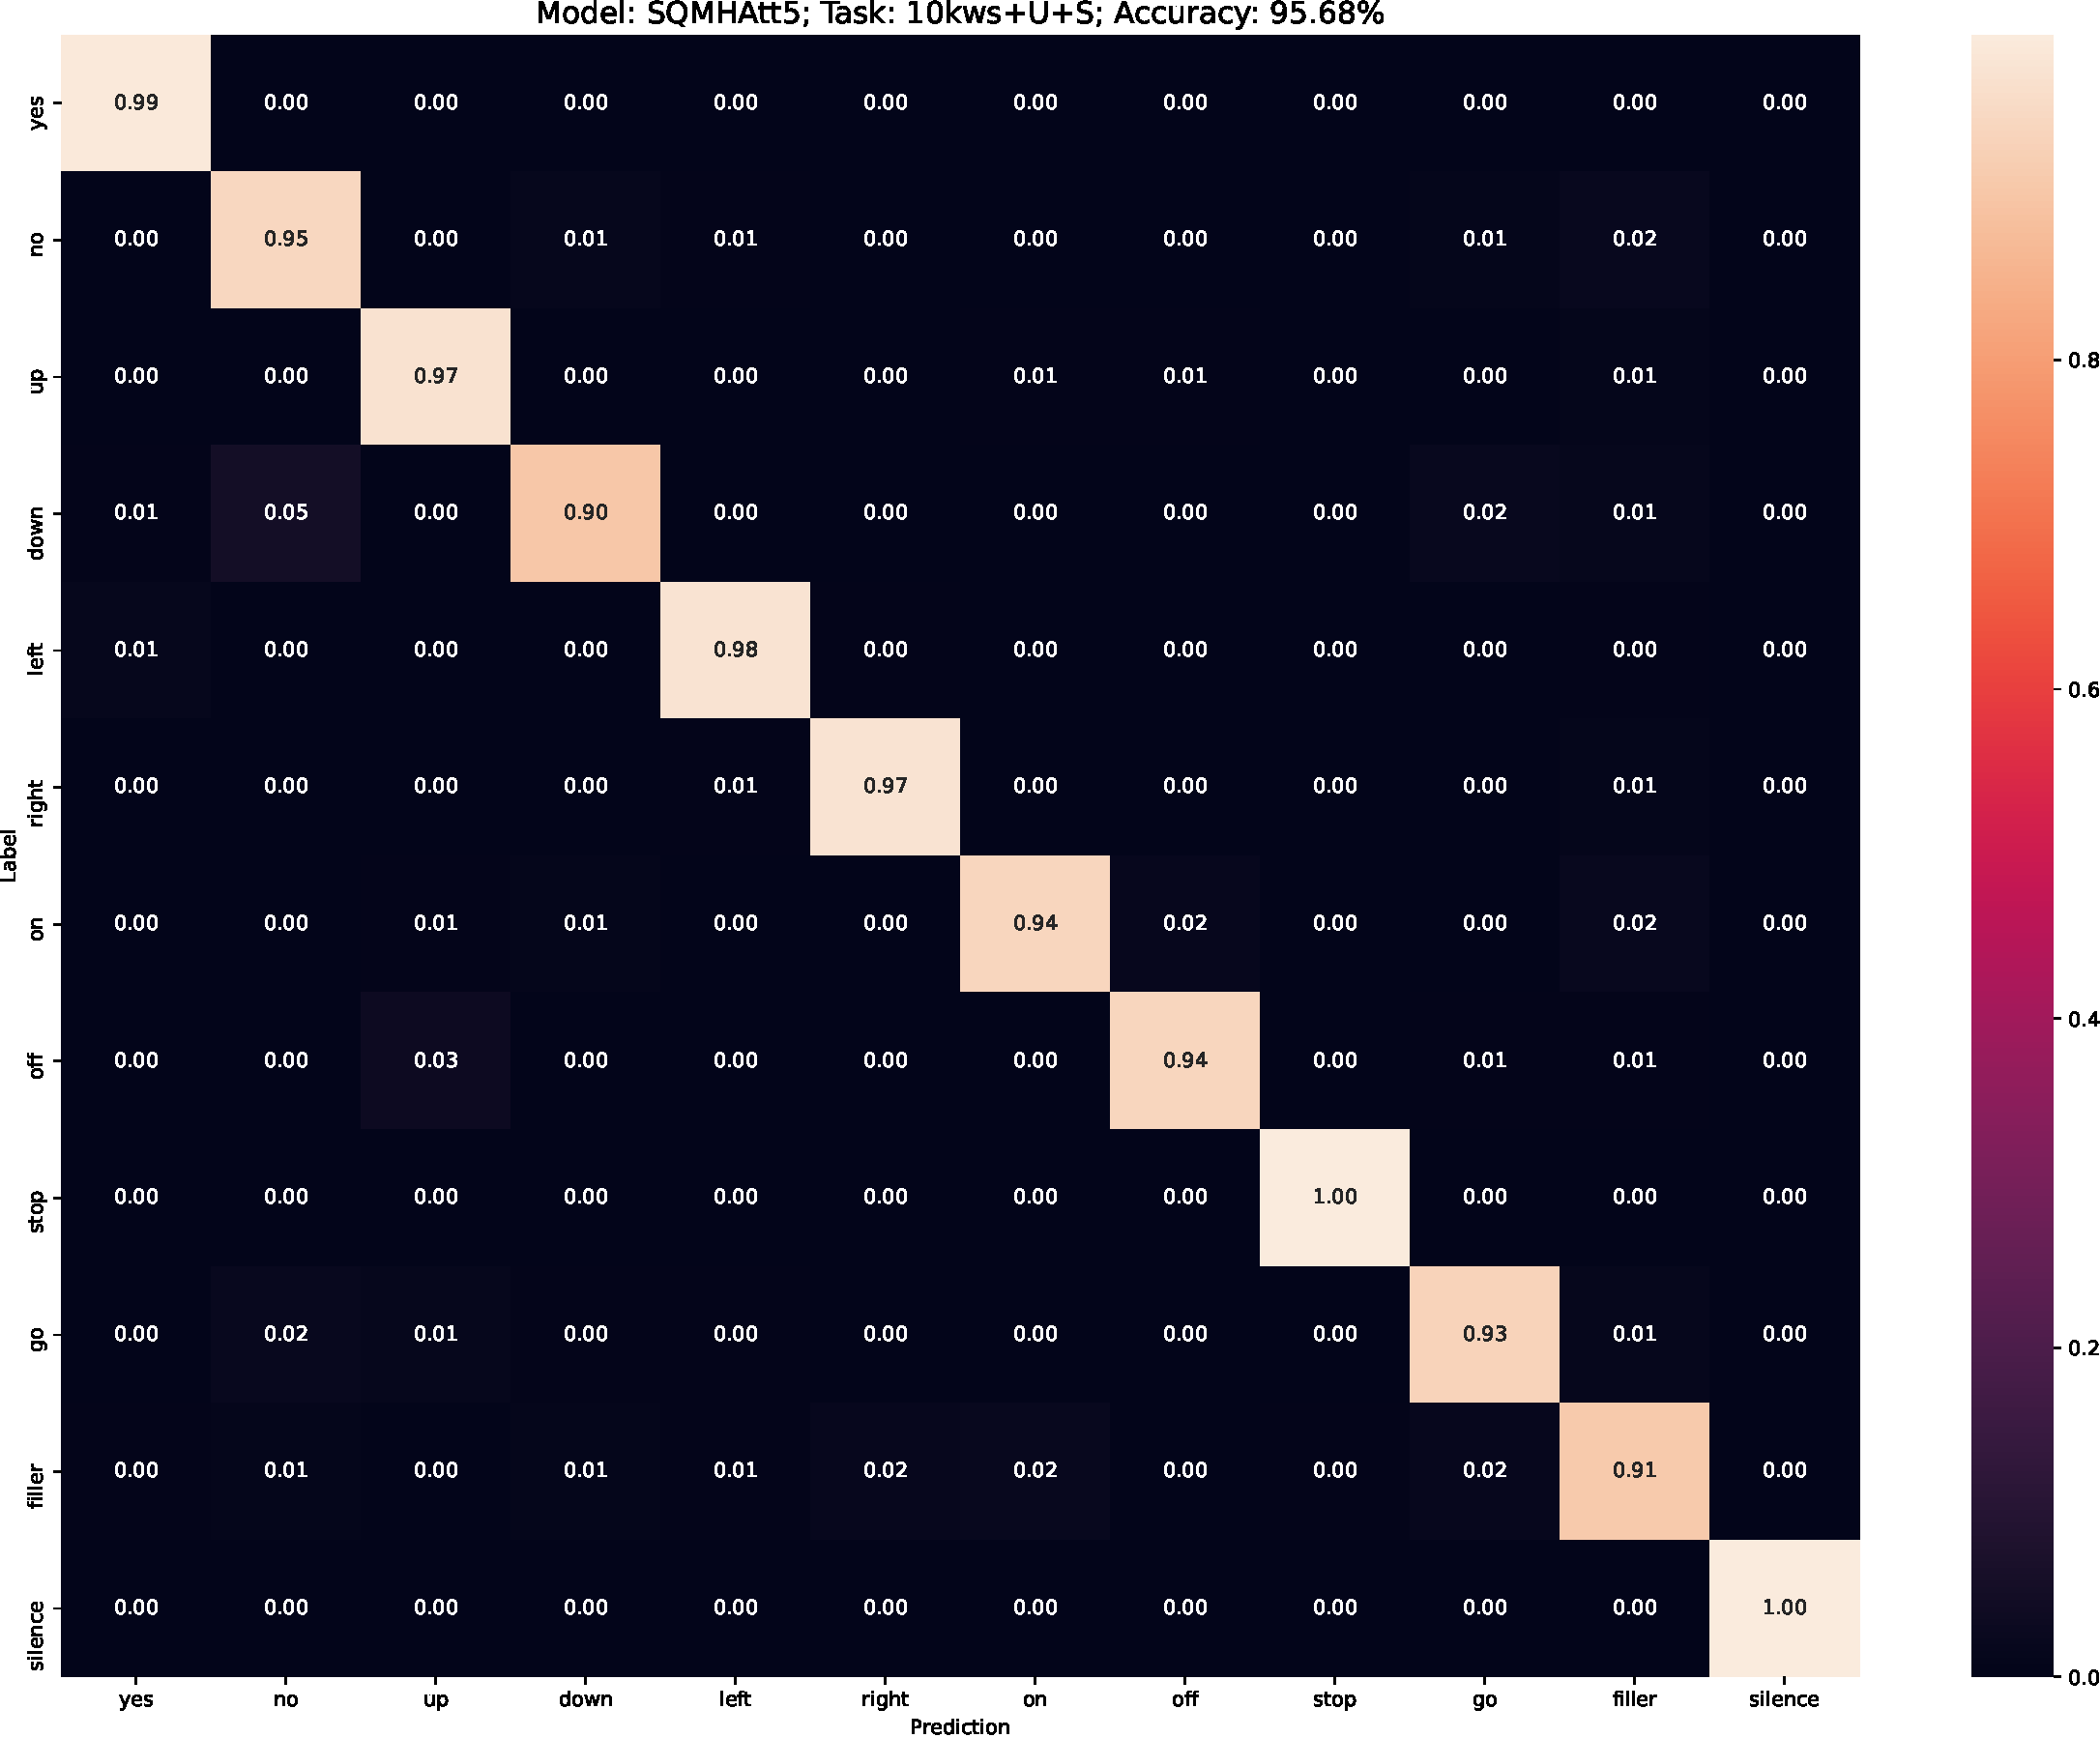
\includegraphics[width=0.8\linewidth]{imgs/SQMHAtt5_12kws.pdf}
		\caption{Confusion matrix of the best performing model for the 12kws task. The words where the model struggle the most are the unknown ones: specifically, known words are often recognized as unknown. Note that this is a desirable situation for a KWS system since we prefer false negatives instead of false positives. Another aspect which should be improved is in the recognition of the word \textit{down}, which is often recognized as \textit{no}.}
%		\label{fig:sub1}
	\end{subfigure}
	\begin{subfigure}{\textwidth}
		\centering

	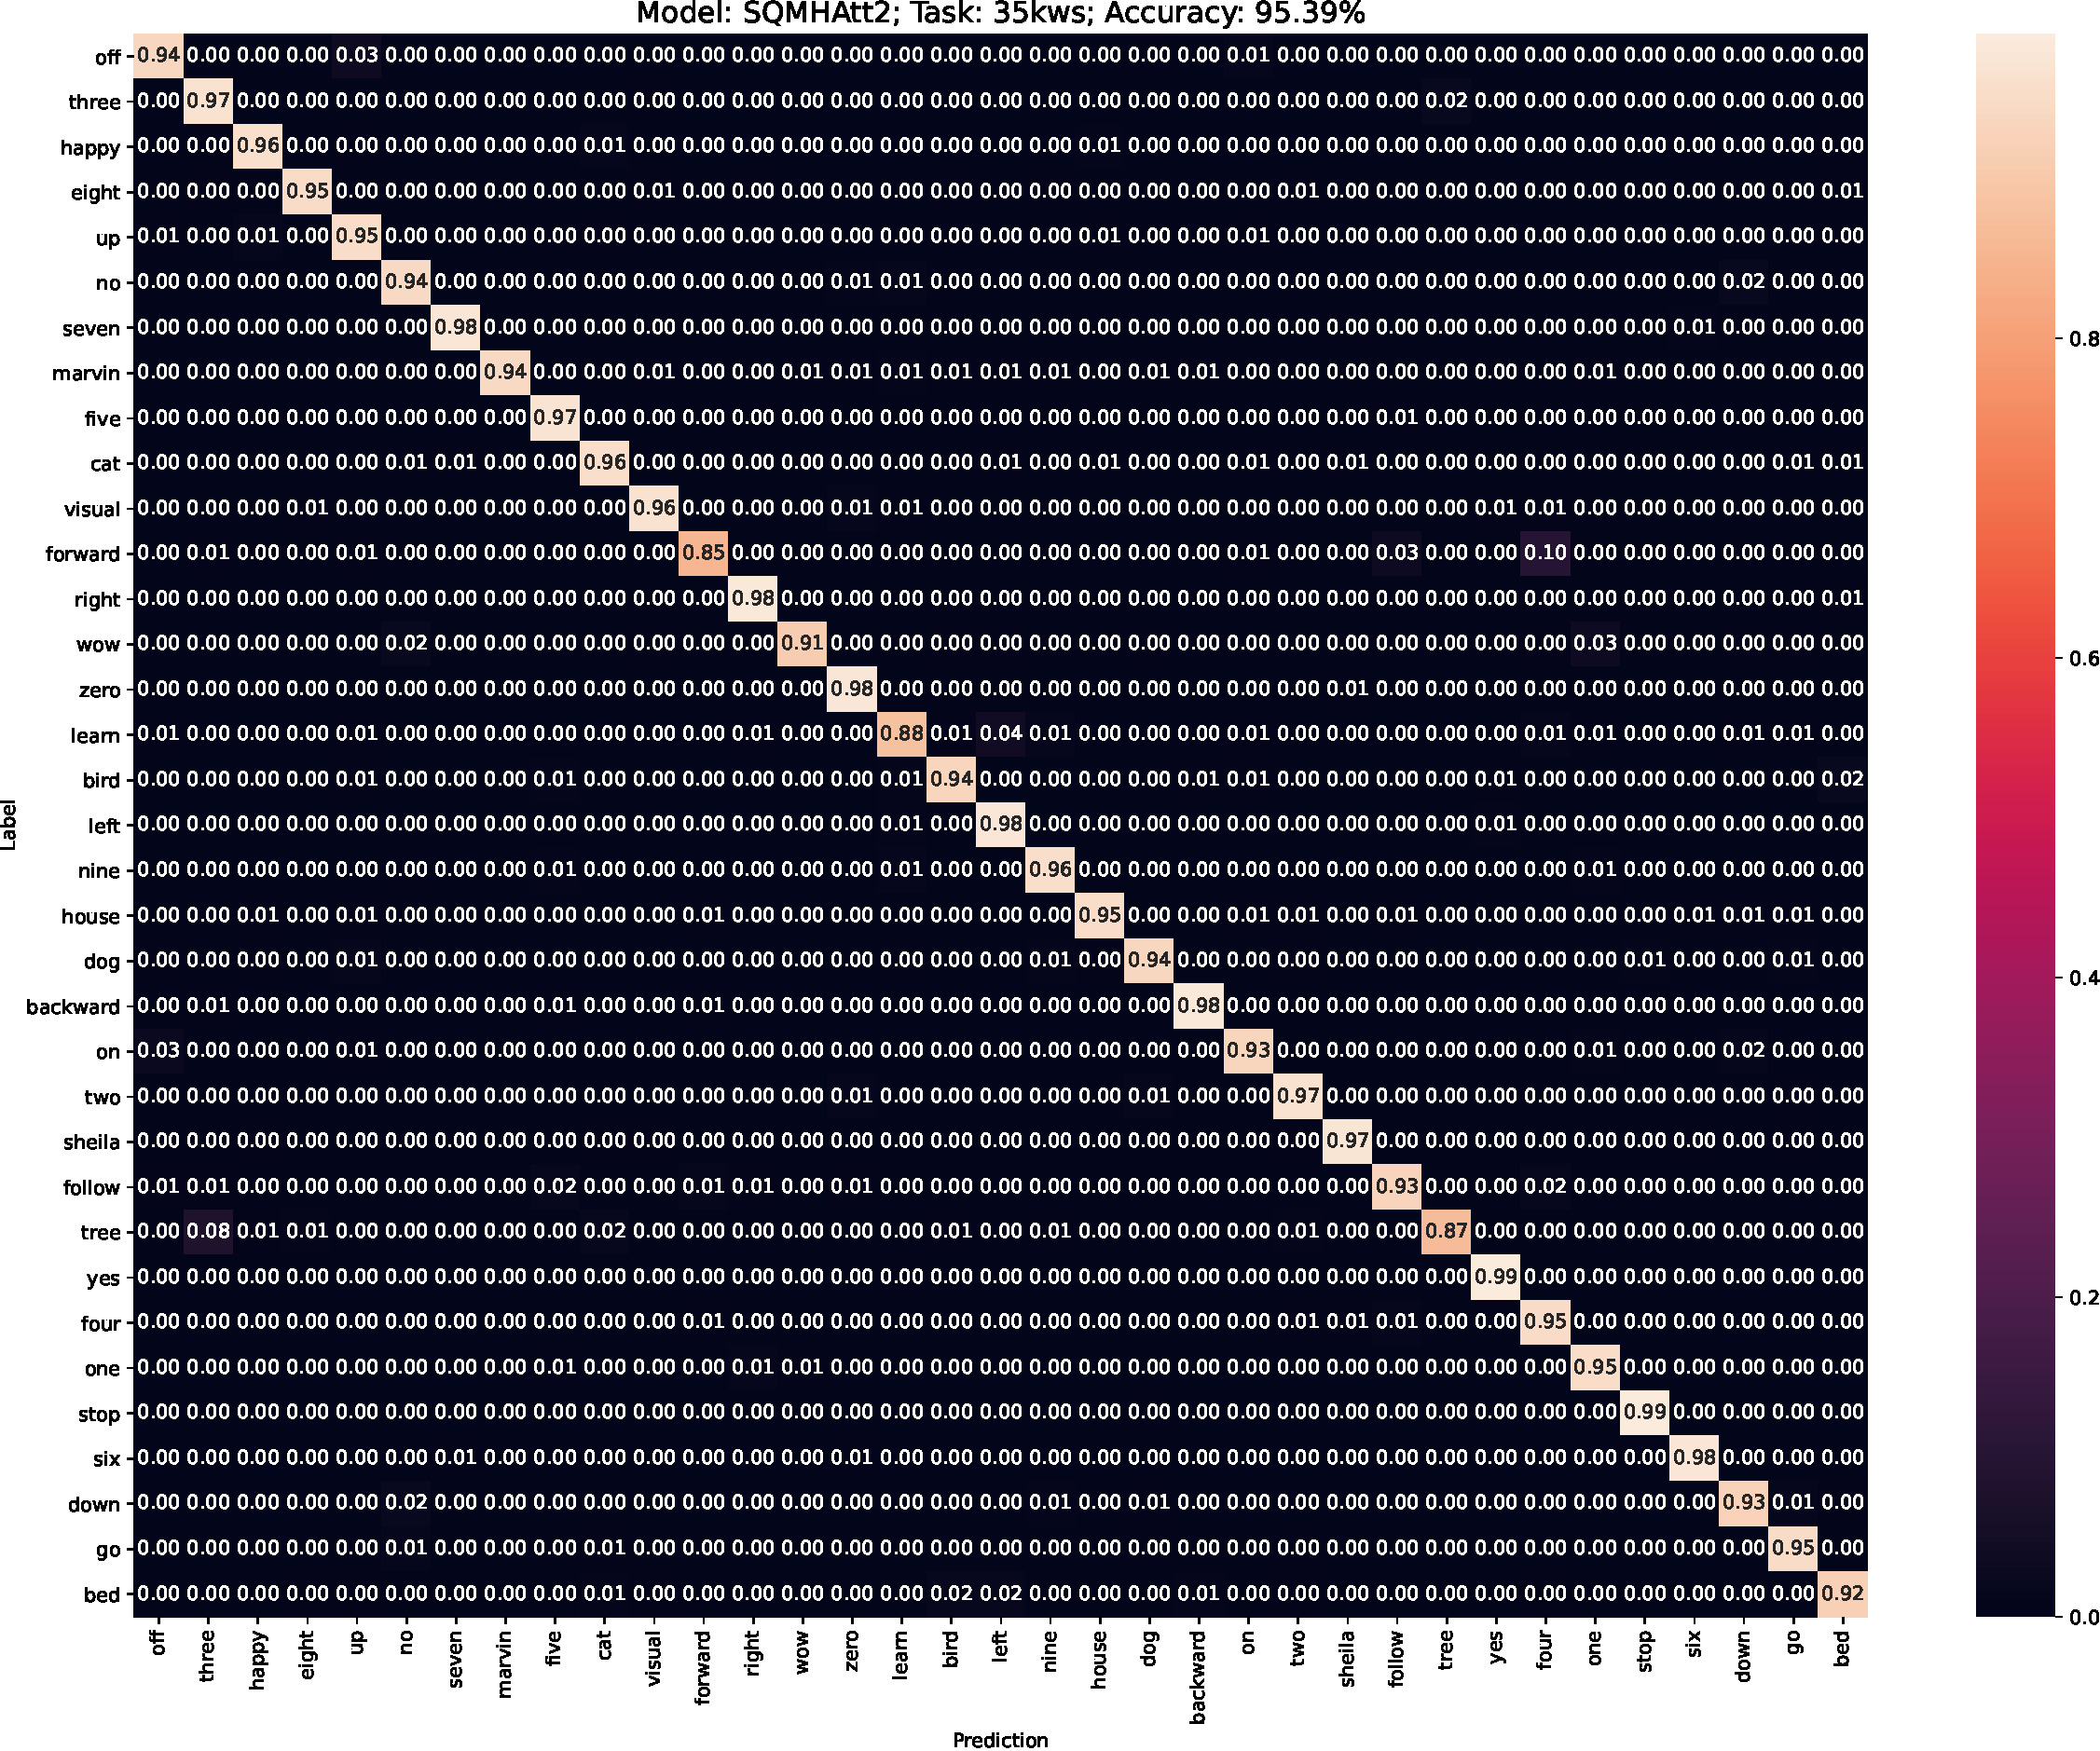
\includegraphics[width=0.8\linewidth]{imgs/SQMHAtt2_35kws.pdf}
			\caption{Confusion matrix of the best performing model for the 35kws task. In this case, two common mistakes can be distinguished. First, the word \textit{forward} is often confused with the word \textit{four}. This is to be expected, since both present the phoneme /\textipa{fOr}/ at the beginning. A similar common error occurs with the word \textit{tree} which is often confused with \textit{three}. Apart from the obvious similarity between the words, another possible reason for this confusion, as pointed by the authors in \cite{attention2018andreade}, might be due to the inability of non native english speakers to correctly pronounce the phoneme  /\textipa{T}/ in \textit{three}.}
%	\label{fig:sub1}
	\end{subfigure}
\end{figure*}



\begin{figure}
	\centering
	\begin{tabular}{cc}
		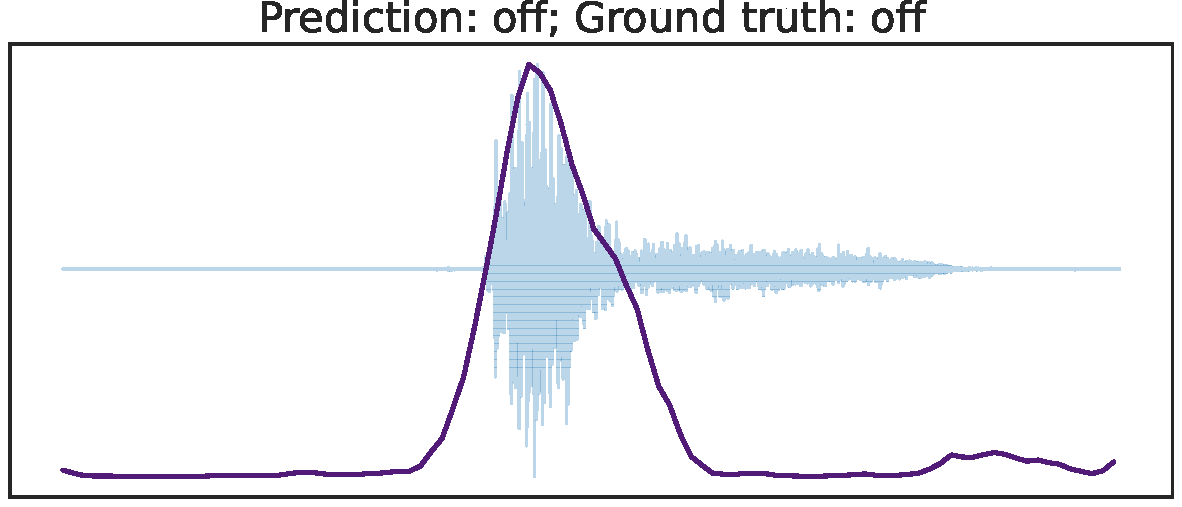
\includegraphics[width = 0.45\linewidth]{imgs/att_scores12_23_andreade.pdf} &
		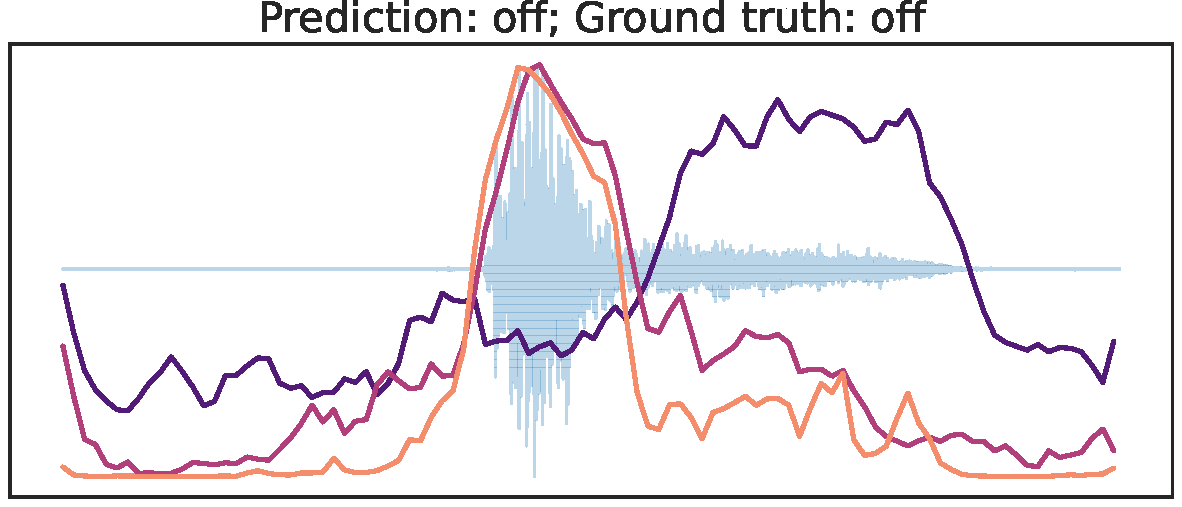
\includegraphics[width = 0.45\linewidth]{imgs/att_scores12_23.pdf}\\
		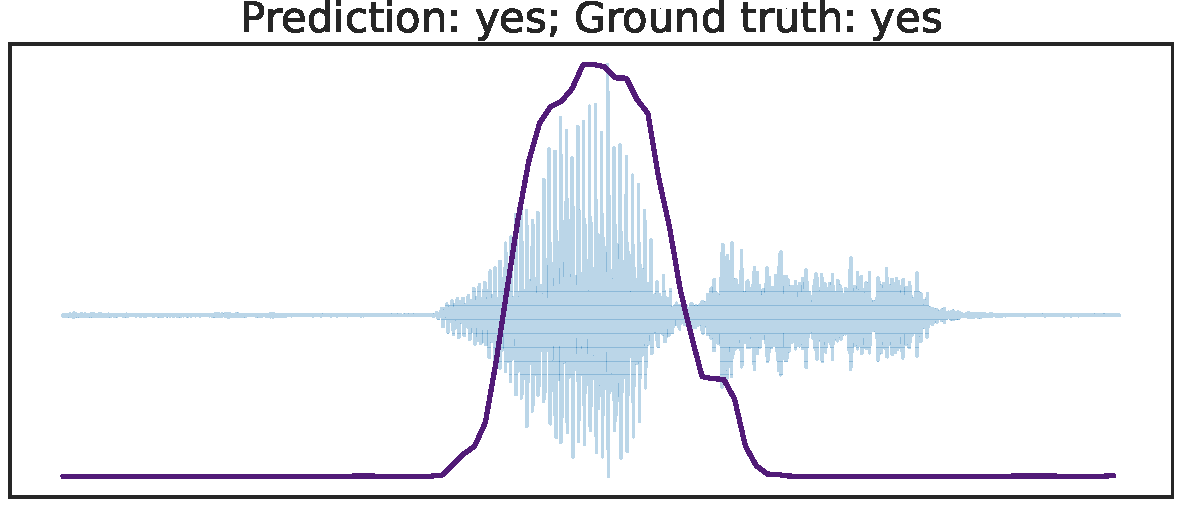
\includegraphics[width = 0.45\linewidth]{imgs/att_scores12_42_andreade.pdf} &
		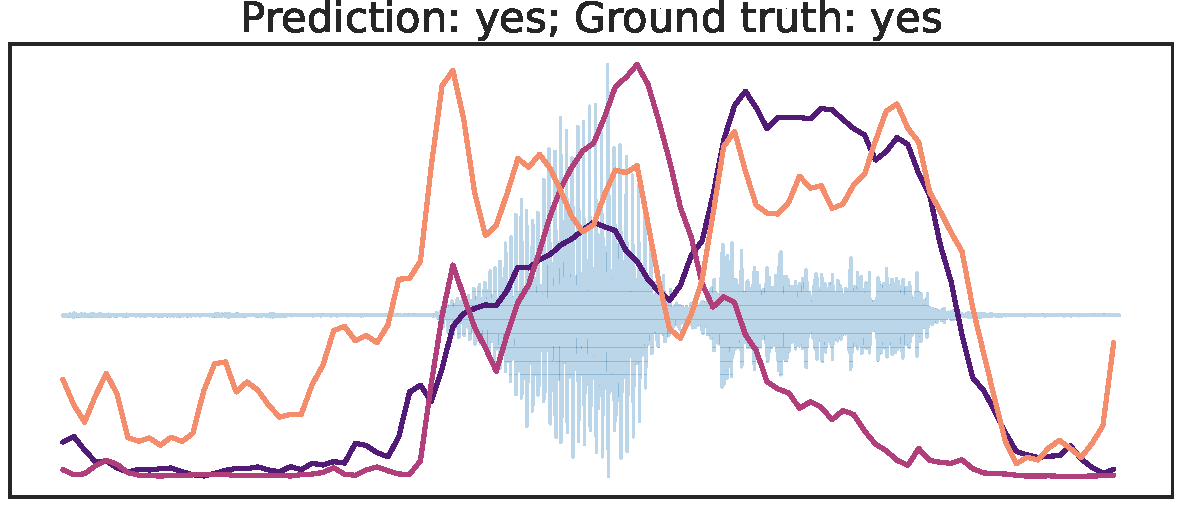
\includegraphics[width = 0.45\linewidth]{imgs/att_scores12_42.pdf}\\
		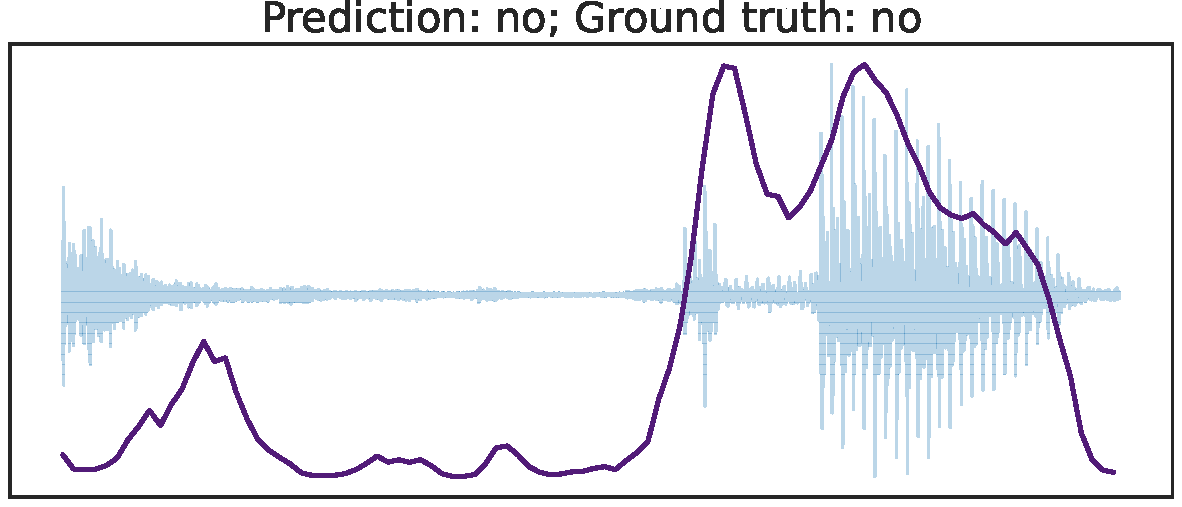
\includegraphics[width = 0.45\linewidth]{imgs/att_scores12_72_andreade.pdf} &
		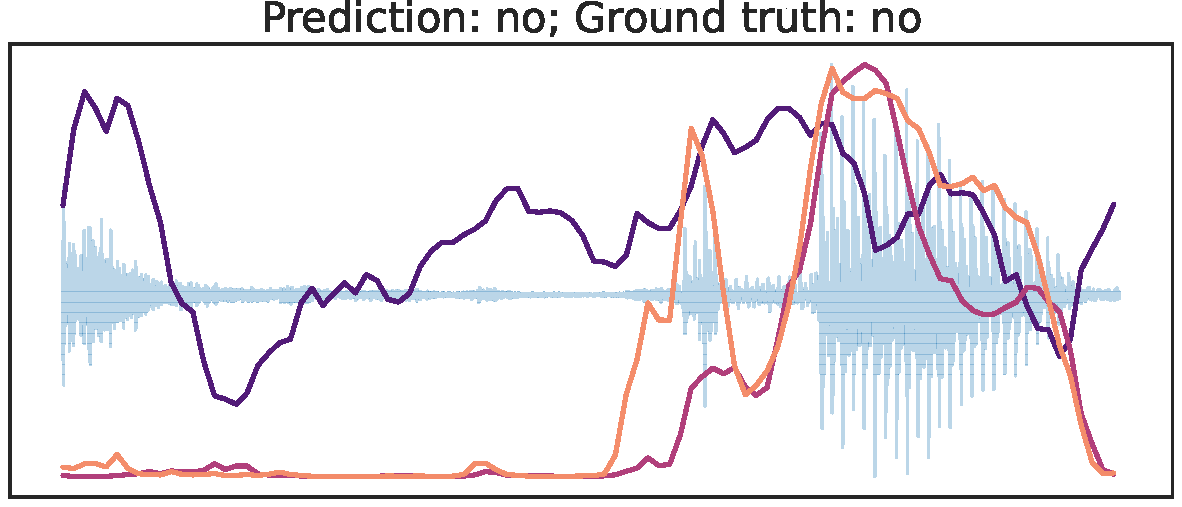
\includegraphics[width = 0.45\linewidth]{imgs/att_scores12_72.pdf}
	\end{tabular}
	\caption{Comparison between attention scores from  Att-RNN model (left) and MHAtt-RNN3 (right), on the words \textit{off}, \textit{yes} and \textit{no}. }
	\label{fig:att_scores}
\end{figure}

\begin{figure*}
	\centering
	\begin{subfigure}{.5\textwidth}
		\centering
		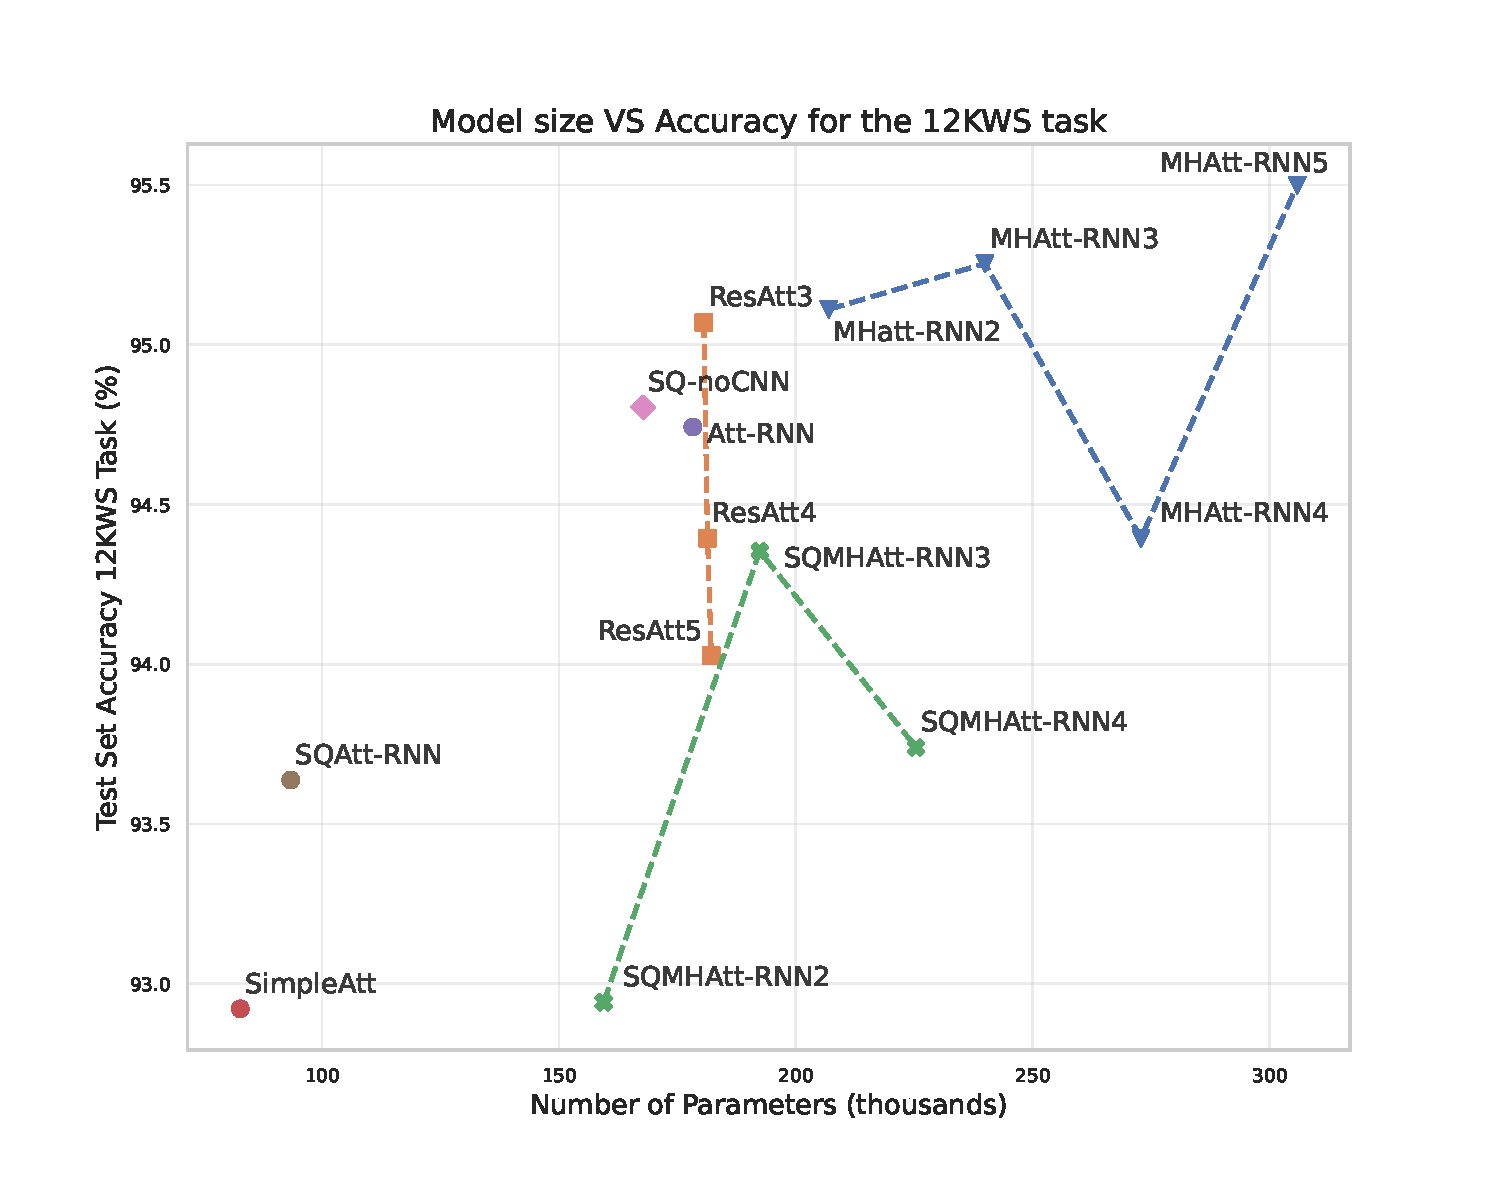
\includegraphics[width=\linewidth]{imgs/size_vs_accuracy12.pdf}
%		\caption{A subfigure}
		\label{fig:sub1}
	\end{subfigure}%
	\begin{subfigure}{.5\textwidth}
		\centering
		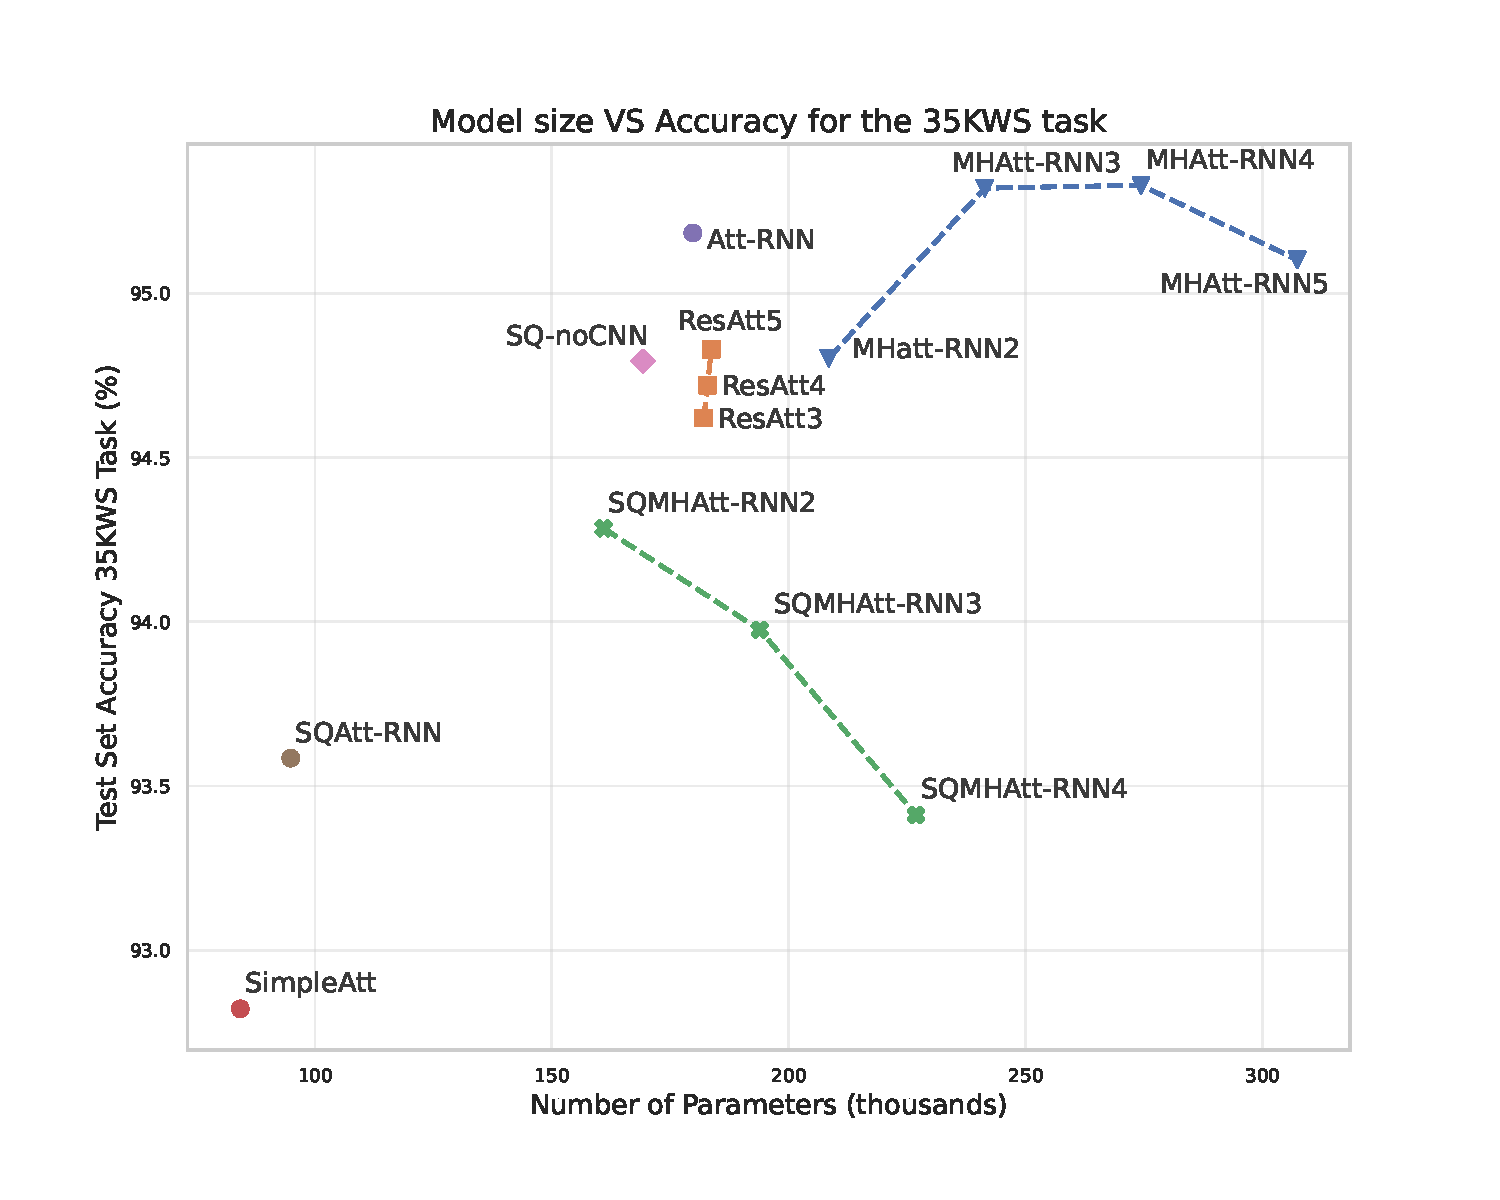
\includegraphics[width=\linewidth]{imgs/size_vs_accuracy35.pdf}
%		\caption{A subfigure}
		\label{fig:sub2}
	\end{subfigure}
	\caption{Models size vs. test set accuracy, for the 12kws (left) and 35kws task (right).}
	\label{fig:accs_vs_parameters}
\end{figure*}

\begin{table}

	\caption{Results in term of top-1 accuracy for both tasks.}

\begin{tabular}{lccc}	
	\hline 
	Model & Param. & Acc. 12kw & Acc. 35kw \\
	\hline \hline
	
	\rule{0pt}{3ex}SimpleAtt & $84 \mathrm{~K}$ & $92.9 \%$ & $92.8 \%$ \\
	Att-RNN & $180 \mathrm{~K}$& $94.7 \%$& $95.2 \%$ \\
	\hline 
	\rule{0pt}{3ex}SQAtt-RNN & $169 \mathrm{~K}$  & $94.9 \%$& $94.6 \%$ \\
	SQAtt-noCNN & $169 \mathrm{~K}$ & $94.8 \%$& $94.8 \%$ \\
	\hline \rule{0pt}{3ex}MHAtt-RNN2 & $208 \mathrm{~K}$ & $95.1 \%$& $94.8 \%$ \\
	MHAtt-RNN3 & $241 \mathrm{~K}$ & $95.2 \%$ & $95.3 \%$\\
	MHAtt-RNN4 & $274 \mathrm{~K}$ & $ 94.4\%$& $95.3 \%$ \\
	MHAtt-RNN5 & $307 \mathrm{~K}$ & $ 95.5\%$& $95.1 \%$ \\
	\hline \rule{0pt}{3ex}SQMHAtt-RNN2 &$235 \mathrm{~K}$ & $95.3 \%$& $\mathbf{95.4} \%$ \\
	SQMHAtt-RNN3 &$268 \mathrm{~K}$ & $95.4 \%$& $94.4 \%$ \\
	SQMHAtt-RNN4& $301 \mathrm{~K}$ & $94.7 \%$& $94.3 \%$ \\
	SQMHAtt-RNN5& $334 \mathrm{~K}$ & $\mathbf{95.7 \%}$& $95.0 \%$ \\
	\hline \rule{0pt}{3ex}Res-AttRNN3 &$182 \mathrm{~K}$ & $95.1\%$& $94.6 \%$ \\
	Res-AttRNN4& $183 \mathrm{~K}$ & $94.4 \%$& $94.7 \%$ \\
	Res-AttRNN5& $184 \mathrm{~K}$ & $94.0\%$& $94.8 \%$ \\
	\hline
	
	\label{table:results}
\end{tabular}
\end{table}
\subsection{Attention Plots}
As already mentioned, a really convenient feature of models based on attention is that it is easy to interpret them. Specifically, we can plot the attention scores of our models to see which portions of the audio files were more important for the model in order to perform inference. In Figure \ref{fig:att_scores} we visualize log attention weights for Att-RNN and MHAtt-RNN3 models. 
We can see that Att-RNN has only one head, so one set of attention scores per prediction is computed. MHAtt-RNN instead computes one set of attention weights per head: here we visualize the attention scores for each head. In these examples, we can see how each head learns to pay attention to different phonemes of the same word. In the first example, Att-RNN pays attention only to the first phoneme /\textipa{o}/, while MHAtt-RNN has two heads paying attention to /o/ and one paying attention to /f/. In the second example, a similar thing happens: Att-RNN pays attention just at the phoneme /\textipa{je}/ while MHAtt-RNN has different heads concentrating both on /\textipa{je}/ and /\textipa{s}/. The third example presents a noise at the beginning which is not part of the spoken word: Att-RNN has its attention drawn a bit, while two of three heads from MHAtt-RNN learn to completely ignore it.


